\documentclass[dvipsnames]{beamer}
\usepackage{CJKutf8}
\usetheme{Madrid}
\usecolortheme{dolphin}
% Prevent undefined bold-italic sans-serif font warnings in beamer
\DeclareFontShape{OT1}{cmss}{bx}{it}{<->ssub * cmss/bx/n}{}
\makeatletter
\setbeamertemplate{footline}{%
  \leavevmode%
  \hbox{%
    \begin{beamercolorbox}[wd=.37\paperwidth,ht=2.25ex,dp=1ex,center]{author in head/foot}%
      \usebeamerfont{author in head/foot}\insertshortauthor\expandafter\ifblank\expandafter{\beamer@shortinstitute}{}{~~(\insertshortinstitute)}
    \end{beamercolorbox}%
    \begin{beamercolorbox}[wd=.37\paperwidth,ht=2.25ex,dp=1ex,center]{title in head/foot}%
      \usebeamerfont{title in head/foot}\insertshorttitle
    \end{beamercolorbox}%
    \begin{beamercolorbox}[wd=.26\paperwidth,ht=2.25ex,dp=1ex,center]{date in head/foot}%
      \usebeamerfont{date in head/foot}\usebeamertemplate{page number in head/foot}\hspace*{2ex}%
    \end{beamercolorbox}}%
  \vskip0pt%
}
\makeatother
\setbeamercolor{titlelike}{bg=Emerald!20, fg=JungleGreen!75!NavyBlue}
\setbeamerfont{title}{series=\bfseries}
%title page
\setbeamercolor{subtitle}{fg=Emerald!70!white}
\setbeamercolor{author}{fg=JungleGreen!80!NavyBlue}
\setbeamercolor{institute}{fg=JungleGreen!80!NavyBlue}
\setbeamercolor{date}{fg=Emerald!70!white}
% footline
\setbeamercolor{footline}{fg=JungleGreen!80!NavyBlue}
\setbeamercolor{author in head/foot}{bg=Emerald!10, fg=JungleGreen!80!NavyBlue}
\setbeamercolor{title in head/foot}{bg=Emerald!18, fg=JungleGreen!80!NavyBlue}
\setbeamercolor{page number in head/foot}{bg=Emerald!25, fg=JungleGreen!60!NavyBlue}
\setbeamercolor{date in head/foot}{fg=Emerald, bg=Emerald!25}
\setbeamercolor{navigation symbols}{fg=NavyBlue!50}
% table of contents / items
\setbeamercolor{structure}{fg=JungleGreen!80!NavyBlue}
\setbeamertemplate{section in toc}[sections numbered]
\setbeamercolor{section in toc}{fg=JungleGreen!80!NavyBlue}
\setbeamercolor{section number projected}{bg=BlueGreen, fg=NavyBlue}
\setbeamercolor{item projected}{bg=BlueGreen, fg=NavyBlue}
\setbeamercolor{item}{fg=JungleGreen!80!NavyBlue}
\setbeamercolor{subitem}{fg=JungleGreen!80!NavyBlue}
\setbeamercolor{subsubitem}{fg=JungleGreen!80!NavyBlue}
\AtBeginDocument{
  \color{JungleGreen!80!NavyBlue}
}

\title{Introduction to MATH1860J}
\subtitle{Prof. Horst Hohberger \& Prof. Luka Zwaan}
\author{Yu Shuhan}
\institute{SJTU Global College}
\date{AC Course Selection Workshop - 2026/9}

\begin{document}

\AtBeginSection[]
{
  {
    \setbeamercolor{background canvas}{bg=Aquamarine!75}
    \setbeamercolor{normal text}{fg=white}
    \setbeamercolor{frametitle}{fg=white}

    \begin{frame}[plain]
      \vfill
      {\bfseries\Large\color{white!60}
        \thesection.~\insertsection

        \vspace{0.3em}
        \noindent
        \textcolor{white}{\rule{0.58\paperwidth}{1pt}}%
        \textcolor{white!45}{\rule{0.27\paperwidth}{1pt}}
      }
      \vfill
    \end{frame}
  }
}

\begin{frame}
    \titlepage
\end{frame}

\begin{frame}{Contents}
    \tableofcontents
\end{frame}

\section{About the Course}
\begin{frame}{Instructor Information: Prof. Horst Hohberger}
    \begin{figure}
    \centering
    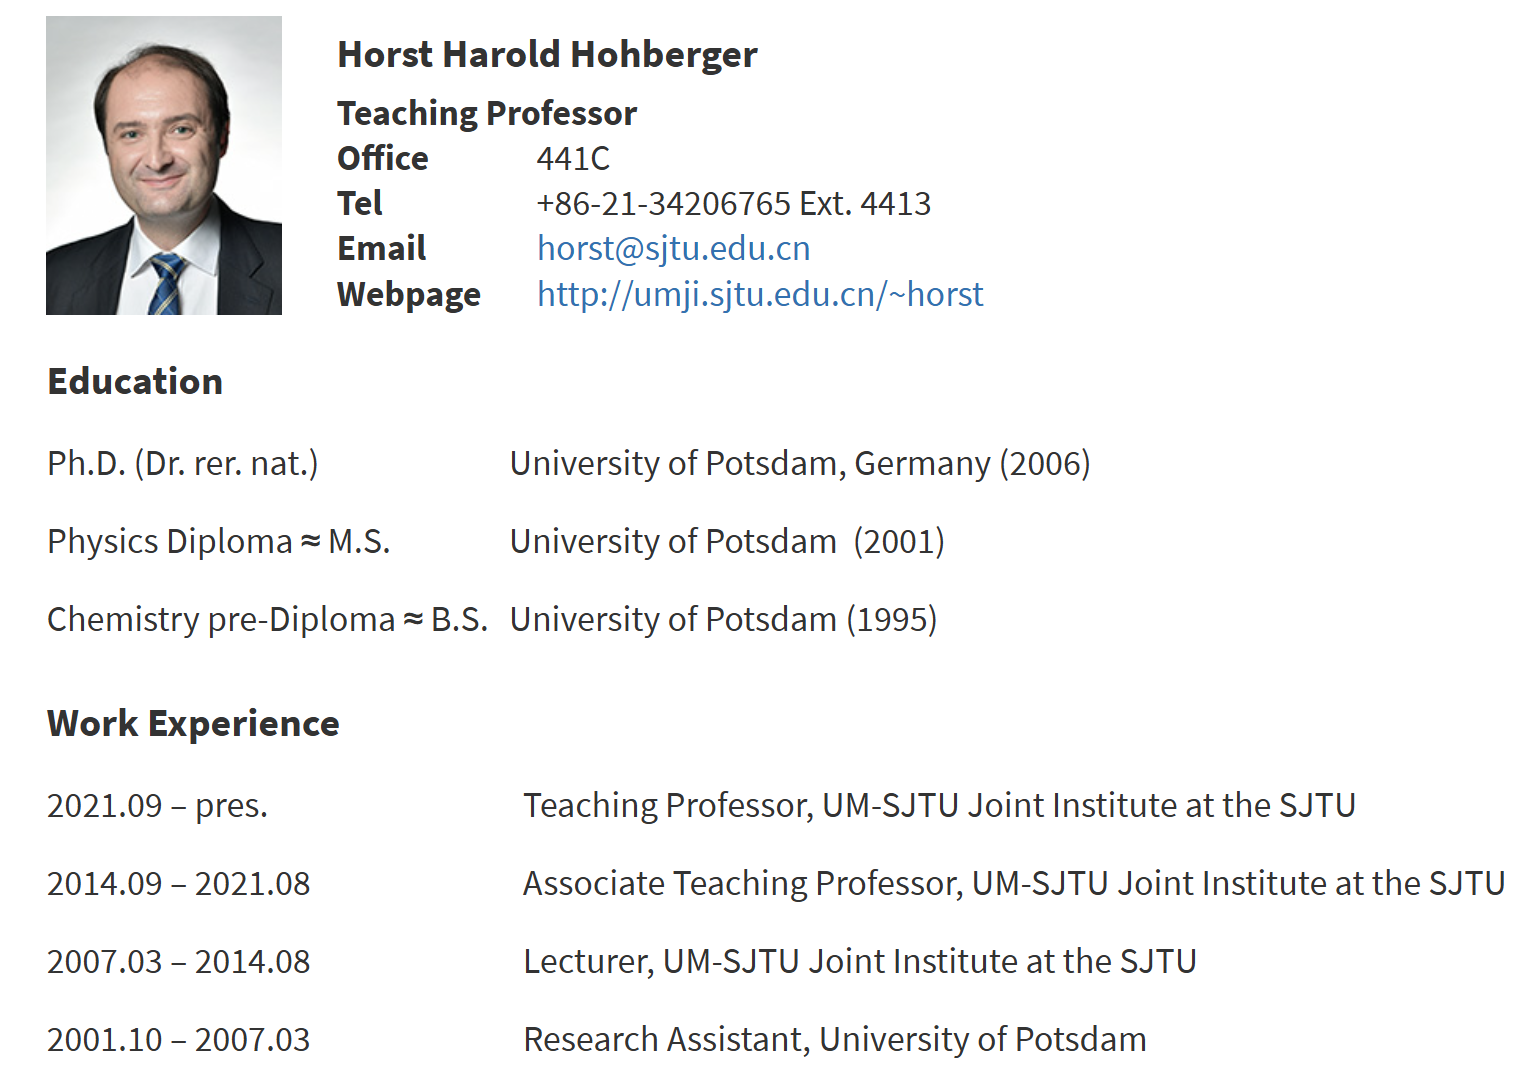
\includegraphics[width=0.78\textwidth]{horst.png}
    \end{figure}
    {\tiny Source: https://gc.sjtu.edu.cn/about/faculty-staff/faculty-directory/}
\end{frame}

\begin{frame}{Instructor Information: Prof. Luka Zwaan}
    \begin{figure}
    \centering
    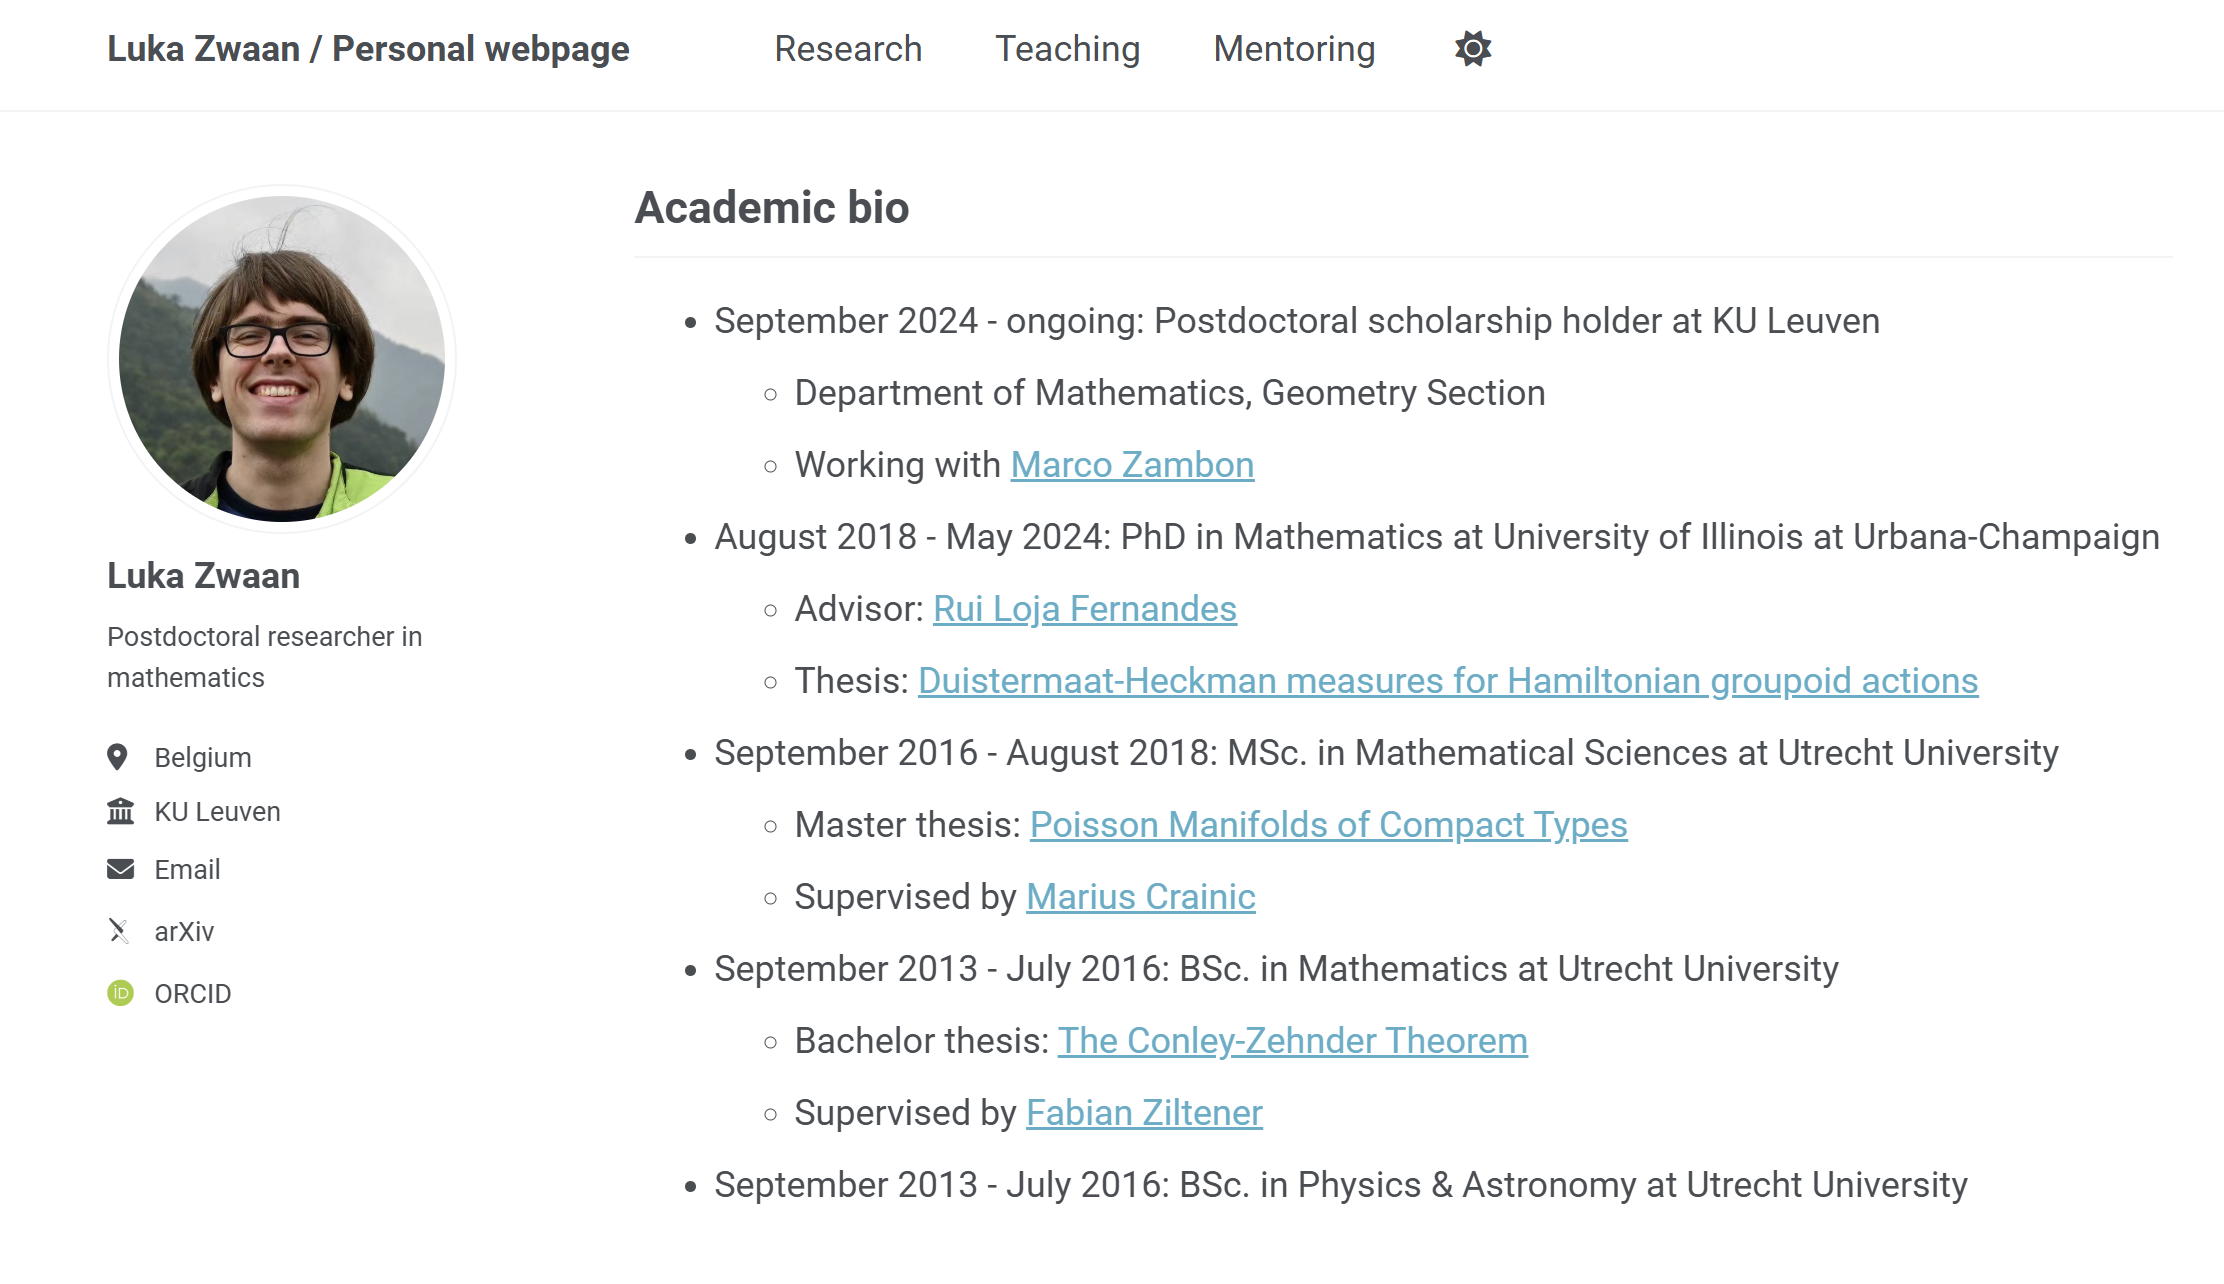
\includegraphics[width=0.9\textwidth]{lukaz.png}
    \end{figure}
    {\tiny Source: https://lukazwaan.github.io/}
\end{frame}

\begin{frame}{Course Overview}
MATH1860J is the first course in the \textit{Honors Mathematics} sequence. It focuses on \textbf{single-variable functions}, with particular emphasis on:
    \begin{itemize}
        \item Mathematic Foundations
        \item Functions, Limits and Continuity
        \item Differentiation, Vector Spaces
        \item Series, Integration and Applications
    \end{itemize}
\vspace{0.3cm}
Friendly Reminders:
    \begin{itemize}
        \item Lectures given by Prof. Hohberger will be online, while those given by Prof. Zwaan will be in-person. Participation in both is encouraged.
        \item Compared to MATH1560J, MATH1860J is more theoretical and abstract. If you are interested in the theoretical induction and rigorous proof of mathematics, this course is for you!
    \end{itemize}
\end{frame}

\begin{frame}{Workload}
    The course workload is moderate to heavy. It requires consistent effort throughout the semester, since you might spend time contemplating the mathematical reasoning. Some assignment problems are also rather challenging to figure out. The workload includes:
    \vspace{0.25cm}
    \begin{itemize}
        \item Lectures: 2.5 * 100 min/week
        \item Recitation Classes: $\approx$ 1 * 120 min/week, led by TAs, not mandatory but recommended.
        \item Assignments: One problem set per week, due the following week. (You will be assigned to an assignment group of 3 students. You are expected to work together with your group members to complete the assignments.)
        \item Midterm and Final Exams Preparation.
    \end{itemize}
\end{frame}

\section{What to Learn \& How to Learn}
\begin{frame}{What to Learn: Course Outcomes}
After completing MATH1860J, students should be able to:
\begin{columns}[T]
    \begin{column}{0.4\textwidth}
        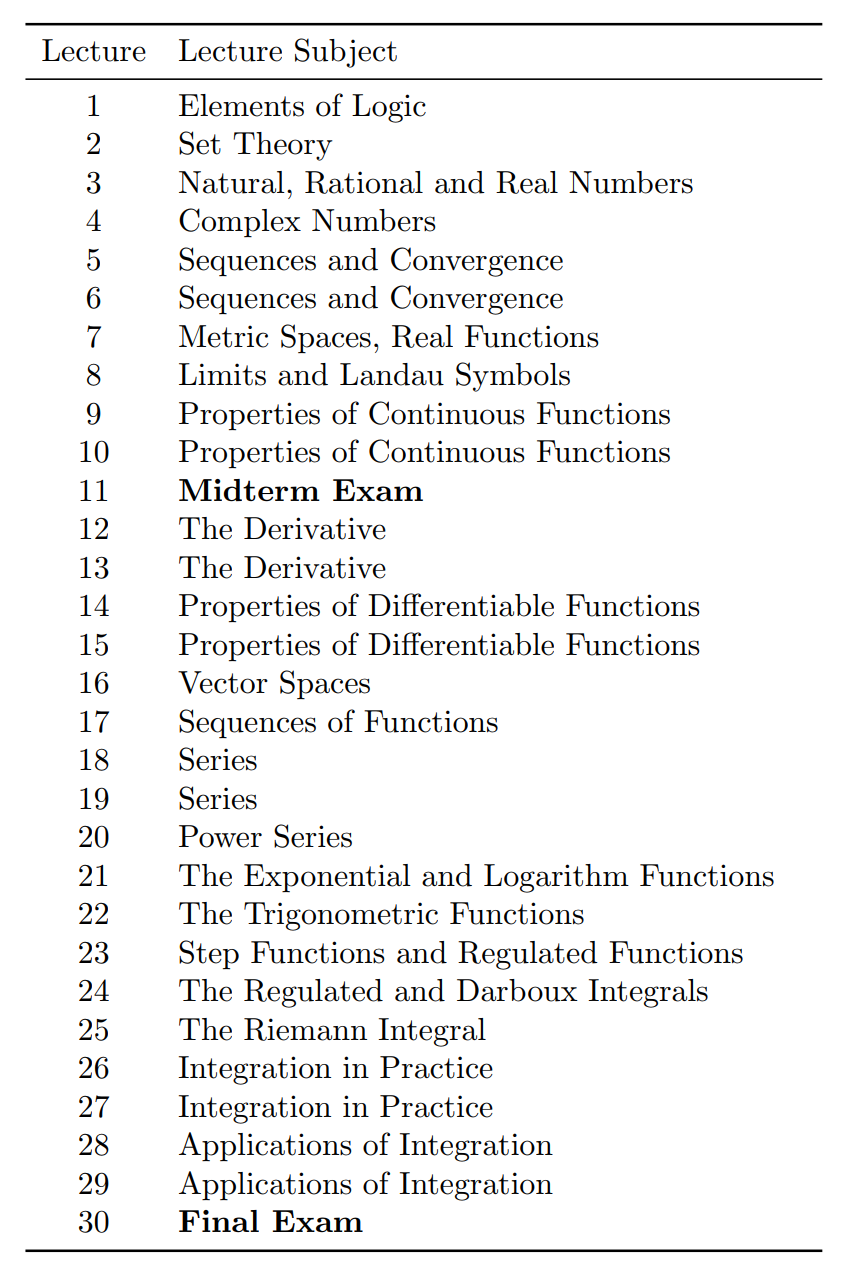
\includegraphics[width=0.95\linewidth]{contents.png}
    \end{column}

    \begin{column}{0.6\textwidth}
        \begin{itemize}
        \item Compute limits of sequences and functions.
        \item Apply continuity and derivative theorems (IVT, MVT, convexity, extrema).
        \item Analyze convergence of series and power series.
        \item Evaluate integrals using various techniques.
        \item Construct and generalize all the outcomes rigorously.
        \item Experience an interesting journey to grasp advanced mathematics.
        \end{itemize}
    \end{column}
\end{columns}
{\tiny Source: MATH186\_course\_description\_2025}
\end{frame}

\begin{frame}{How to Learn It Well I}
Differences between Elementary Math and Advanced Math:
\begin{itemize}
    \item Define concepts clearly $\to$ Certainty.
    \item Use what is certain to model real-world problems $\to$ Modeling.
    \item Generalize and prove with mathematical tools $\to$ Thinking.
\end{itemize}

\vspace{0.5cm}
``I'm good at math in high school'' $\not\Leftrightarrow$ ``I learn VV186/MATH1860J well.''

\vspace{0.5cm}

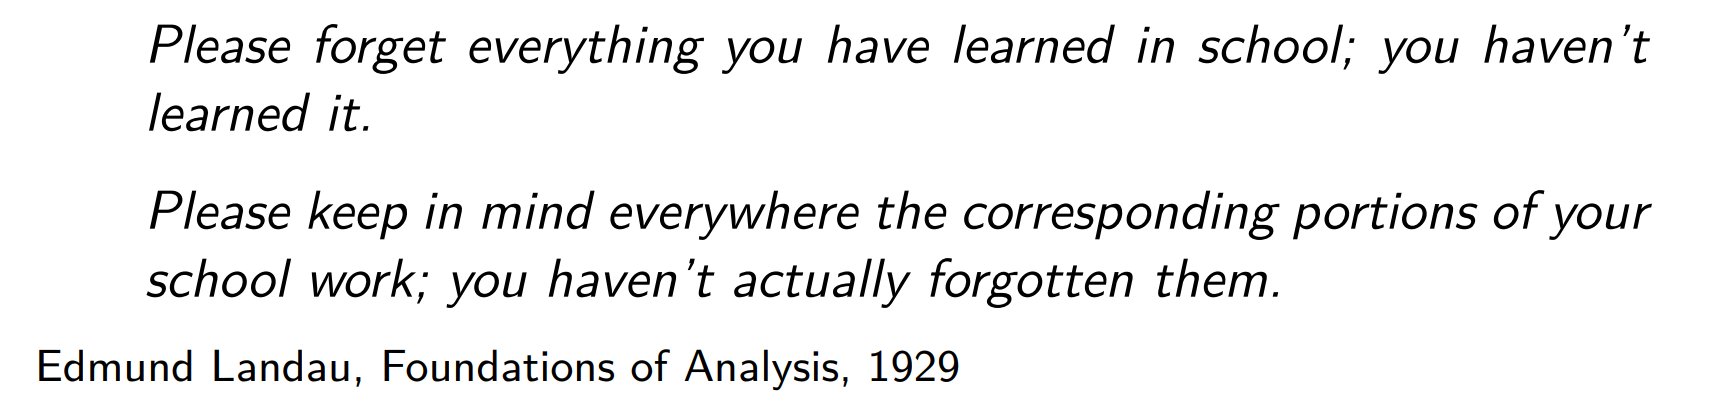
\includegraphics[width=0.95\linewidth]{quote.png}
\end{frame}

\begin{frame}{How to Learn It Well II}
    TAs' Suggestions:
    \begin{itemize}
        \item Attend lectures and follow the instructor's pace. Focus on key points and general ideas instead of memorizing every detail.
        \item Preview and review the lecture slides carefully, make sure you grasp every concept, theorem and definition, and understand the proof.
        \item Get familiar with mathematical analytical expression and notation. Don't be afraid of the abstractness of advanced mathematics.
        \item Do the assignments, quizzes and sample exams by yourself. Don't overrely on provided solutions or AI.
        \item Attending recitation classes (RCs) might help you to organize the knowledge framework.
        \item Actively discuss with your classmates. Post your questions on piazza.
        \item You could always ask for help from our kind TAs and instructors during office hours. Don't hesitate to ask questions!
    \end{itemize}
\end{frame}

\section{Student Feedback}
\begin{frame}[allowframebreaks]{Comments on This Course}
    \begin{quote}
        \color{NavyBlue}
    ``Math186 is a really interesting course, where you obtain a lot while suffering from its abstract parts. However, enjoy your journey with 186 and remember to "bother" your TAs when suffering. \textbf{When you suffer, rush to canvas-files-sample\_exams.}''
    \end{quote}
    \vspace{0.5em}
    \begin{quote}
        \color{Emerald}
    ``Math186 is more similar to ``Mathematics analysis'', which focuses more on how to proof and why the theorems work, instead of how to calculate the results. It is more abstract than 156 and harder to get started. But when you get familiar with those concepts and terms, you will find the beauty of math.''
    \end{quote}
    \vspace{0.5em}
    \begin{quote}
        \normalfont
        \color{NavyBlue}
        \begin{CJK}{UTF8}{gbsn}
    “一门需要抛弃高中知识从头开始学的课（hst语），但是186不像想象中‘纯证明’那么难，认真做作业和sample exam还是可以拿到不错的分数的。”
    \end{CJK}
    \end{quote}
    \vspace{0.5em}
    \begin{quote}
        \color{Emerald}
    ``Perfect course, perfect professor. Your effort will certainly pay off as long as you really dive into the course and learn it by heart.''
    \end{quote}
    \vspace{0.5em}
    \begin{quote}
        \normalfont
        \color{NavyBlue}
        \begin{CJK}{UTF8}{gbsn}
    “数分是一个很值得沉下心认真学习的课，只要愿意认认真真学习，不断积累沉淀，可以拿到一个不错的分数！”
    \end{CJK}
    \end{quote}
    \vspace{0.5em}
    \begin{quote}
        \normalfont
        \color{Emerald}
        \begin{CJK}{UTF8}{gbsn}
    “不知道我会不会是比较负面的回答。可能怪我自己学习方法和态度的问题。不只是186，很多JI课程我都是那种临时抱佛脚的状态。尽管最后成绩还算可以，但是对我来说，我其实并没有学到很多知识，基本都是考试前能对这门课的整个知识点有个大概的掌握，但是到了下学期，我对于这些知识会忘记很多。可能是我自己的学习问题，不过个人对于186的学习经历还挺负面的。”
        \end{CJK}
    \end{quote}
\end{frame}

\section{Grading}
\begin{frame}{Grading Policy in 25FA}
    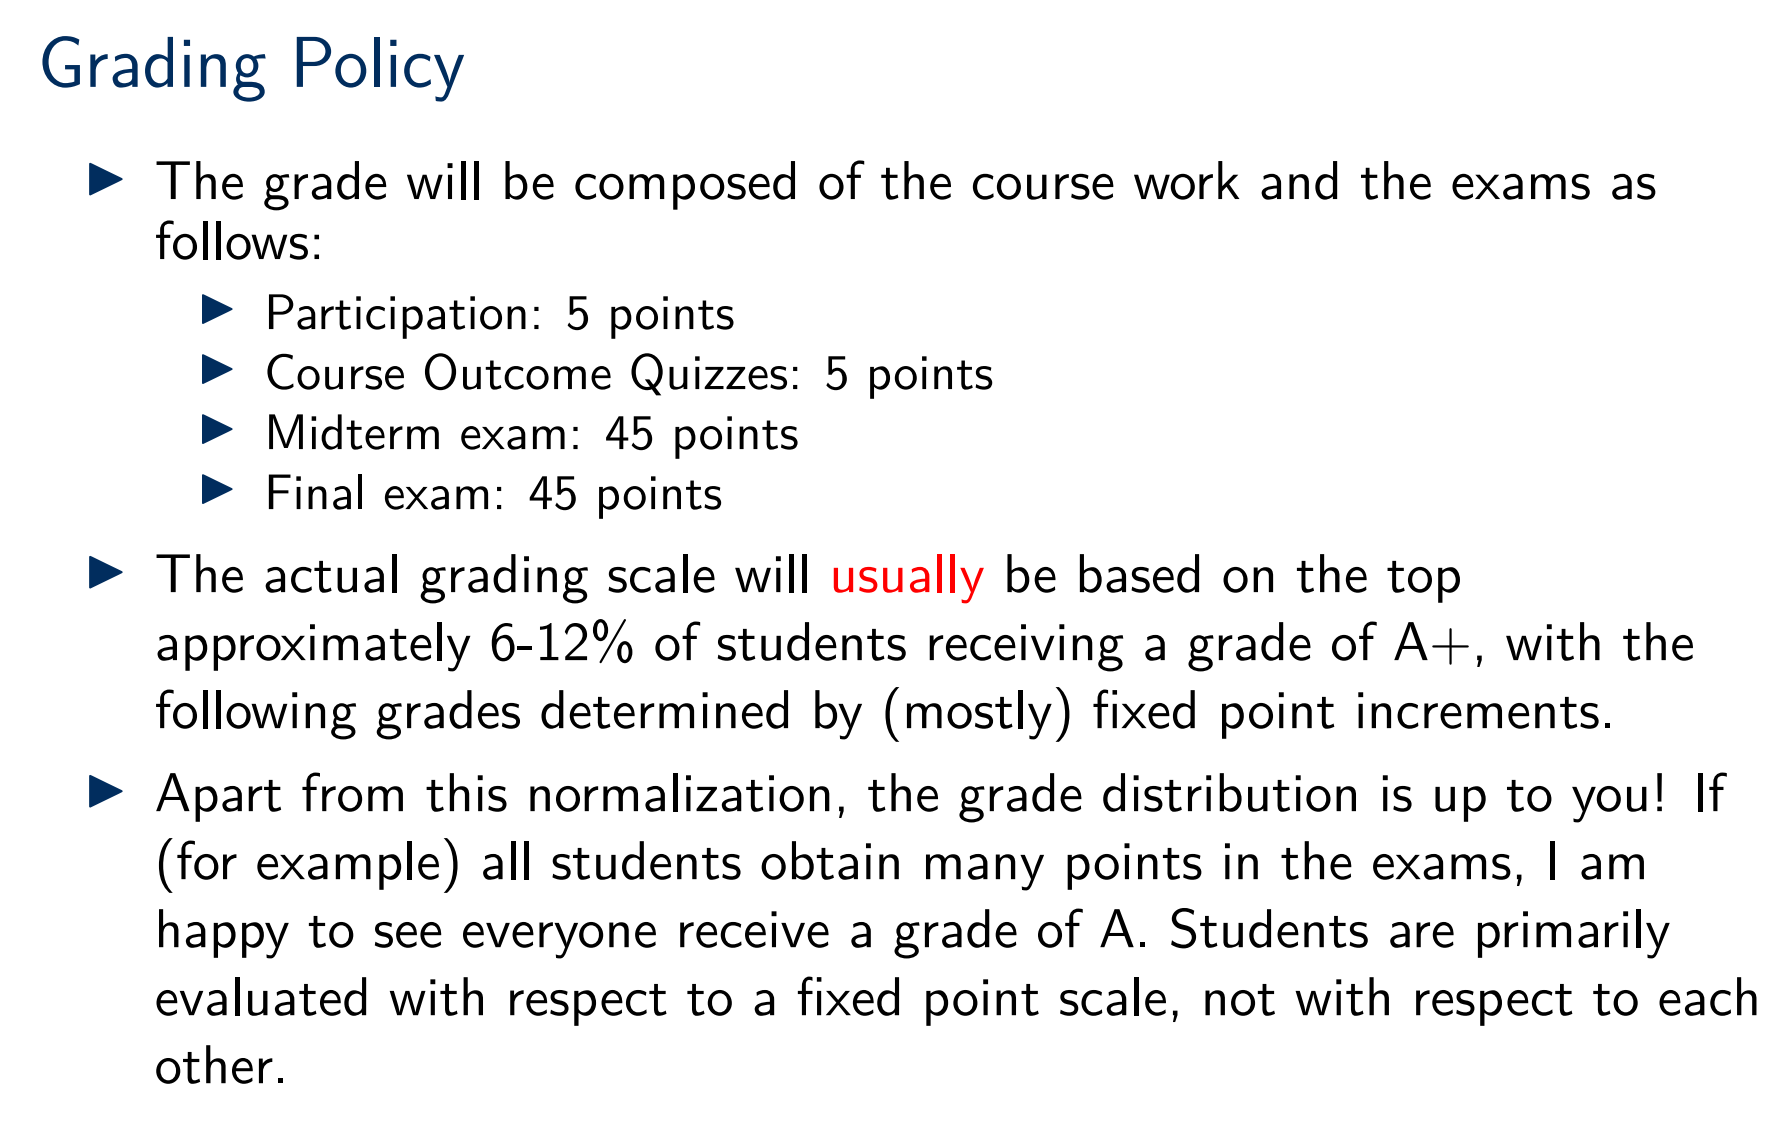
\includegraphics[width=0.95\linewidth]{grading.png}
    {\tiny Source: math186\_all\_lecture\_slides}
\end{frame}

\section{Contact}
\begin{frame}{Contact}
\begin{columns}[c]
    \begin{column}{0.4\textwidth}
        \flushright
        You could reach out to us MATH1860J TAs via email, WeChat or Feishu. \\
        You could also join the unofficial Q \& A group chat if you have any questions or concerns about the course.
    \end{column}
    \begin{column}{0.6\textwidth}
        \centering
        
\includegraphics[width=0.7\linewidth]{group.jpg}
    \end{column}
\end{columns}
\end{frame}

\begin{frame}{References}
\begin{itemize}
  \item Horst Hohberger, \textit{math186\_all\_lecture\_slides (2025)}
  \item MATH186\_course\_description\_2025
  \item Wenxin Chen, \textit{Introduction to Vv186}, AC Course Selection Workshop - 2025/9
\end{itemize}
\end{frame}

\section{Q \& A Session}
\begin{frame}
    \centering \huge Thanks for Listening! \\
    \vspace{0.5cm}
    \centering \large Any questions? Please feel free to ask!
\end{frame}

\end{document}